\documentclass{assignment}
\begin{document}

\title{5370 Midterm}

\textbf{1.} A random variable $X$ has the same probability of one third at the points $x=-1,0,1.$  Its entropy is thus $H_X = \log_2 3.$ Let $g(\cdot) $ denote a continuous function and define the random variable $Y=g(X)$.
\begin{enumerate}
\item  Find a continuous function, $g(\cdot )$, that reduces the entropy of $Y$ to zero. \\
  \textbf{Solution:} \\
  $g = \sin(\pi x)$
  \begin{figure}[!h]
  \centering
  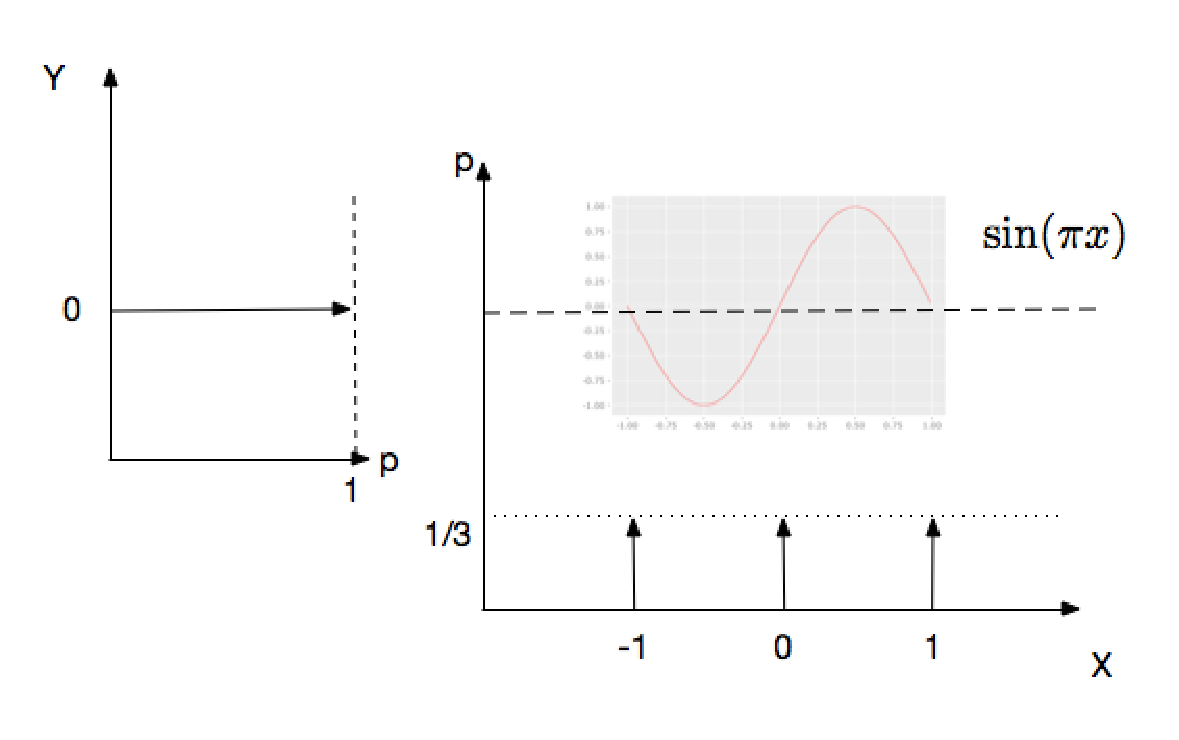
\includegraphics[width=5in]{pics/problem1a.eps}
  \caption{Figure for problem1a}
  \label{fig:problem1a}
  \end{figure}

\item  Find another continuous function, $g(\cdot )$, that reduces the entropy of $Y$ below the entropy of $X$,
  but not to zero. \\
  \textbf{Solution:} \\
  $g = |x|$
  \begin{figure}[!h]
  \centering
  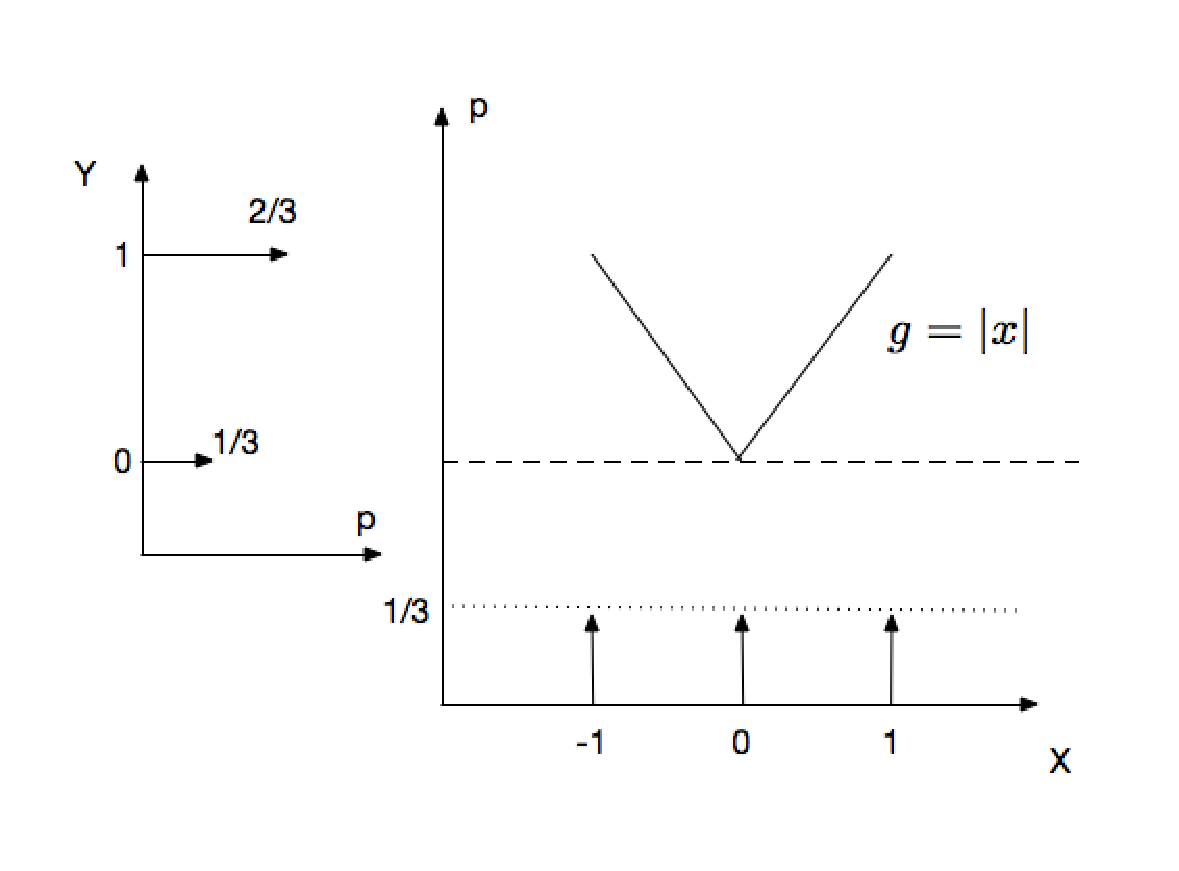
\includegraphics[width=5in]{pics/problem1b.eps}
  \caption{Figure for problem1b}
  \label{fig:problem1b}
  \end{figure}

\item  Find a third function , $g(\cdot )$, that generates an entropy of $Y$ equal to the entropy of $X$.\\
  \textbf{Solution:} \\
  $g = x + 1$
  \begin{figure}[!h]
  \centering
  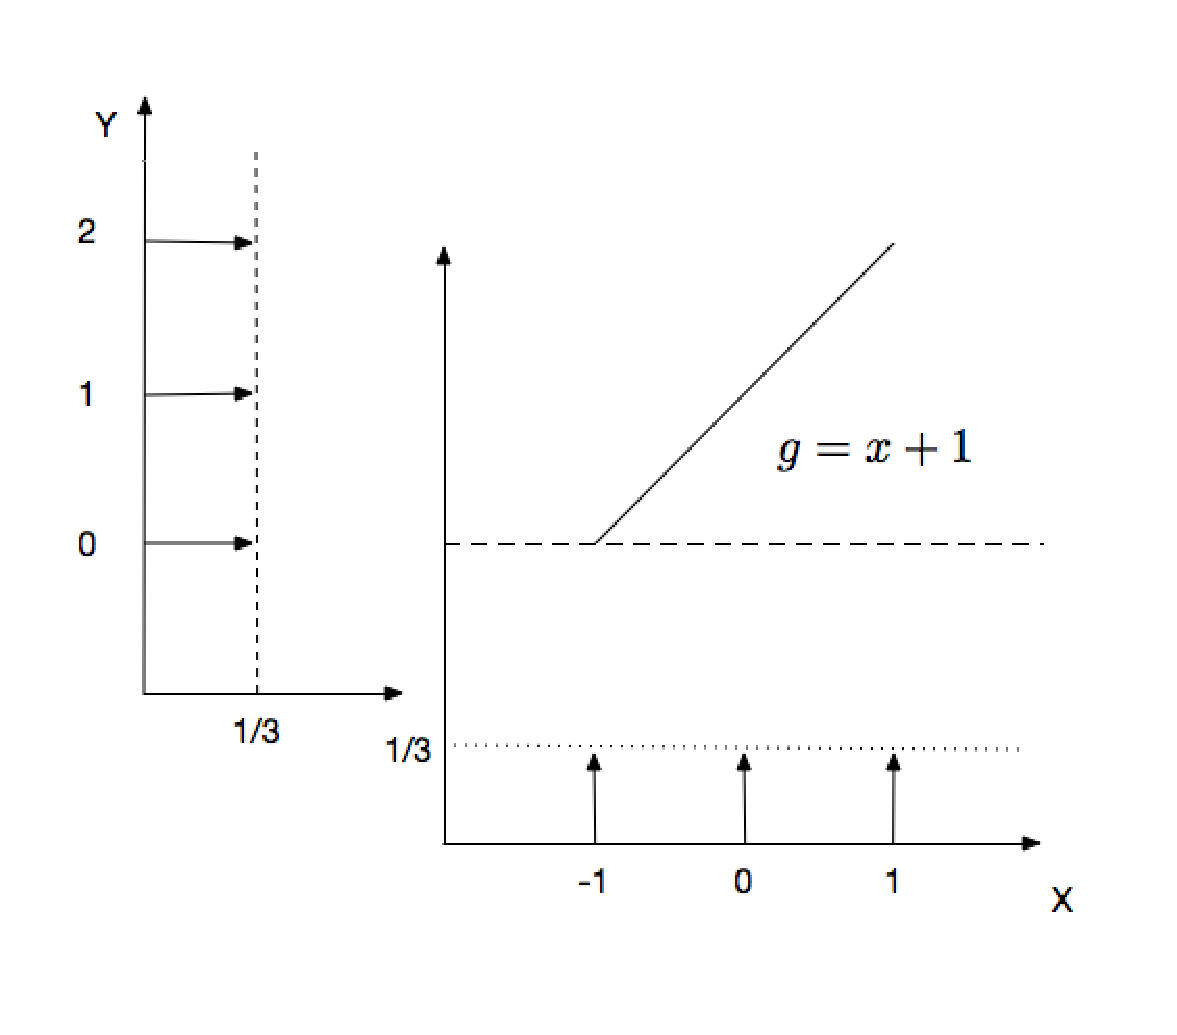
\includegraphics[width=5in]{pics/problem1c.eps}
  \caption{Figure for problem1c}
  \label{fig:problem1c}
  \end{figure}

\end{enumerate}
For all three answers, please sketch the nonlinearity and label your axes.


\end{document}